%
% Kapitel: Foobar
%

\chapter{Foobar}
Wer testet, der questet.\cite{bib:vodafone-legt-in-pirmasens}


% Figure
\begin{nicepic}
    
\includegraphics[width=0.9\textwidth]{images/stars.jpg}
    \captionof{figure}{Sterne}
    \caption*{Quelle: \cite{bib:vodafone-legt-in-pirmasens}}
    \label{fig:stars}
\end{nicepic}

% Multifigure
\begin{figure}[!htbp]
    \begin{subfigure}[t]{0.3\textwidth}
        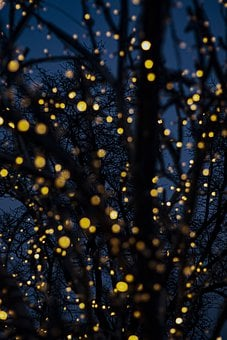
\includegraphics[width=\textwidth]{images/mult0.jpg}
        \captionof{figure}{Lichtpunkte auf dunklem Hintergrund}
        \caption*{Quelle: \cite{bib:vodafone-legt-in-pirmasens}}
        \label{fig:light-points-on-dark-bg}
    \end{subfigure}
    \hfill
    \begin{subfigure}[t]{0.3\textwidth}
        
\includegraphics[width=\textwidth]{images/mult1.png}
        \captionof{figure}{Ein Tannenbaum}
        \caption*{Quelle: \cite{bib:vodafone-legt-in-pirmasens}}
        \label{fig:tannenbaum}
    \end{subfigure}
    \hfill
    \begin{subfigure}[t]{0.3\textwidth}
        
\includegraphics[width=\textwidth]{images/mult2.jpg}
        \captionof{figure}{Eine Winterstadt}
        \caption*{Quelle: \cite{bib:vodafone-legt-in-pirmasens}}
        \label{fig:winter-city}
    \end{subfigure}


    \caption{Ein Beispiel für mehrere Bilder nebeneinander}
\end{figure}

% Table
\begin{table}[!htbp] % !htbp soll wohl das Objekt möglichst nah zum Text-punkt halten
    \centering
    \begin{tabular}{|l|l|r|}
        \hline
        \textbf{TM Configuration}   &   \textbf{Detail-Level}   &   \textbf{Frametime}\\
        \hline
        \hline
        Tensor-800                  &   0                       &   28\\
        Tensor-800                  &   1                       &   52\\
        Tensor-800                  &   2                       &   69\\
        Tensor-800                  &   3                       &   89\\
        \hdashline
        V-Core Zenyx 33             &   0                       &   2\\
        V-Core Zenyx 33             &   1                       &   4\\
        V-Core Zenyx 33             &   2                       &   5\\
        V-Core Zenyx 33             &   3                       &   7\\
        \hdashline
        Intel iZ237-8               &   0                       &   298\\
        Intel iZ237-8               &   1                       &   448\\
        Intel iZ237-8               &   2                       &   556\\
        Intel iZ237-8               &   3                       &   767\\
        \hline
    \end{tabular}
    \caption{Renderzeiten mit TM-Prozessoren}
    \label{tbl:renderzeiten_tm_processors}
\end{table}
